% Chapter Template

\chapter{Introduction} % Main chapter title

\noindent\textbf{\large Contents:}

\noindent\hrulefill
\noindent\startcontents[chapters]
\noindent\printcontents[chapters]{}{1}{}
\noindent\hrulefill

\label{Chapter1} % Change X to a consecutive number; for referencing this chapter elsewhere, use \ref{ChapterX}

Advances in astronomy come in many forms, from the exploration of new theories to new observational techniques.
But astronomy would not be possible without the main tool of the astronomer, the telescope.  Starting from when
Galileo Galilei first pointed his telescope to the night sky, astronomers have been demanding more from their
telescopes.  The only way to enhance a telescopes resolving power is to increase the primary aperture of the
telescope.  In the early 1900's telescopes were made up of a large single optics for the primary aperture. 
However, there is a limit to how large you can make a single optic.  

Eventually, these mirrors were becoming so
large that the mirrors would sag under their own weight.  These large optics quickly became heavier and needed
more mechanical supports.  In order to solve this problem, a honeycomb substructure was designed to keep the
mirrors lighter and more ridged.  Figure \ref{fig:hale} shows the primary mirror of the 200-inch Hale telescope
and backlight to show the structure.  While this helped keep large single optics rigid, there is still a limit
to how large one optic can be.  The University of Arizona's Large Optics Facility is capable of constructing
8.4 meter mirrors \cite{LOFTSystems.}.  One of the reasons for this limit is that this is roughly the maximum
width of bridge underpasses in Arizona.  In order to achieve larger primary apertures, a different approach is
needed.


\begin{figure}[!h]
\centering
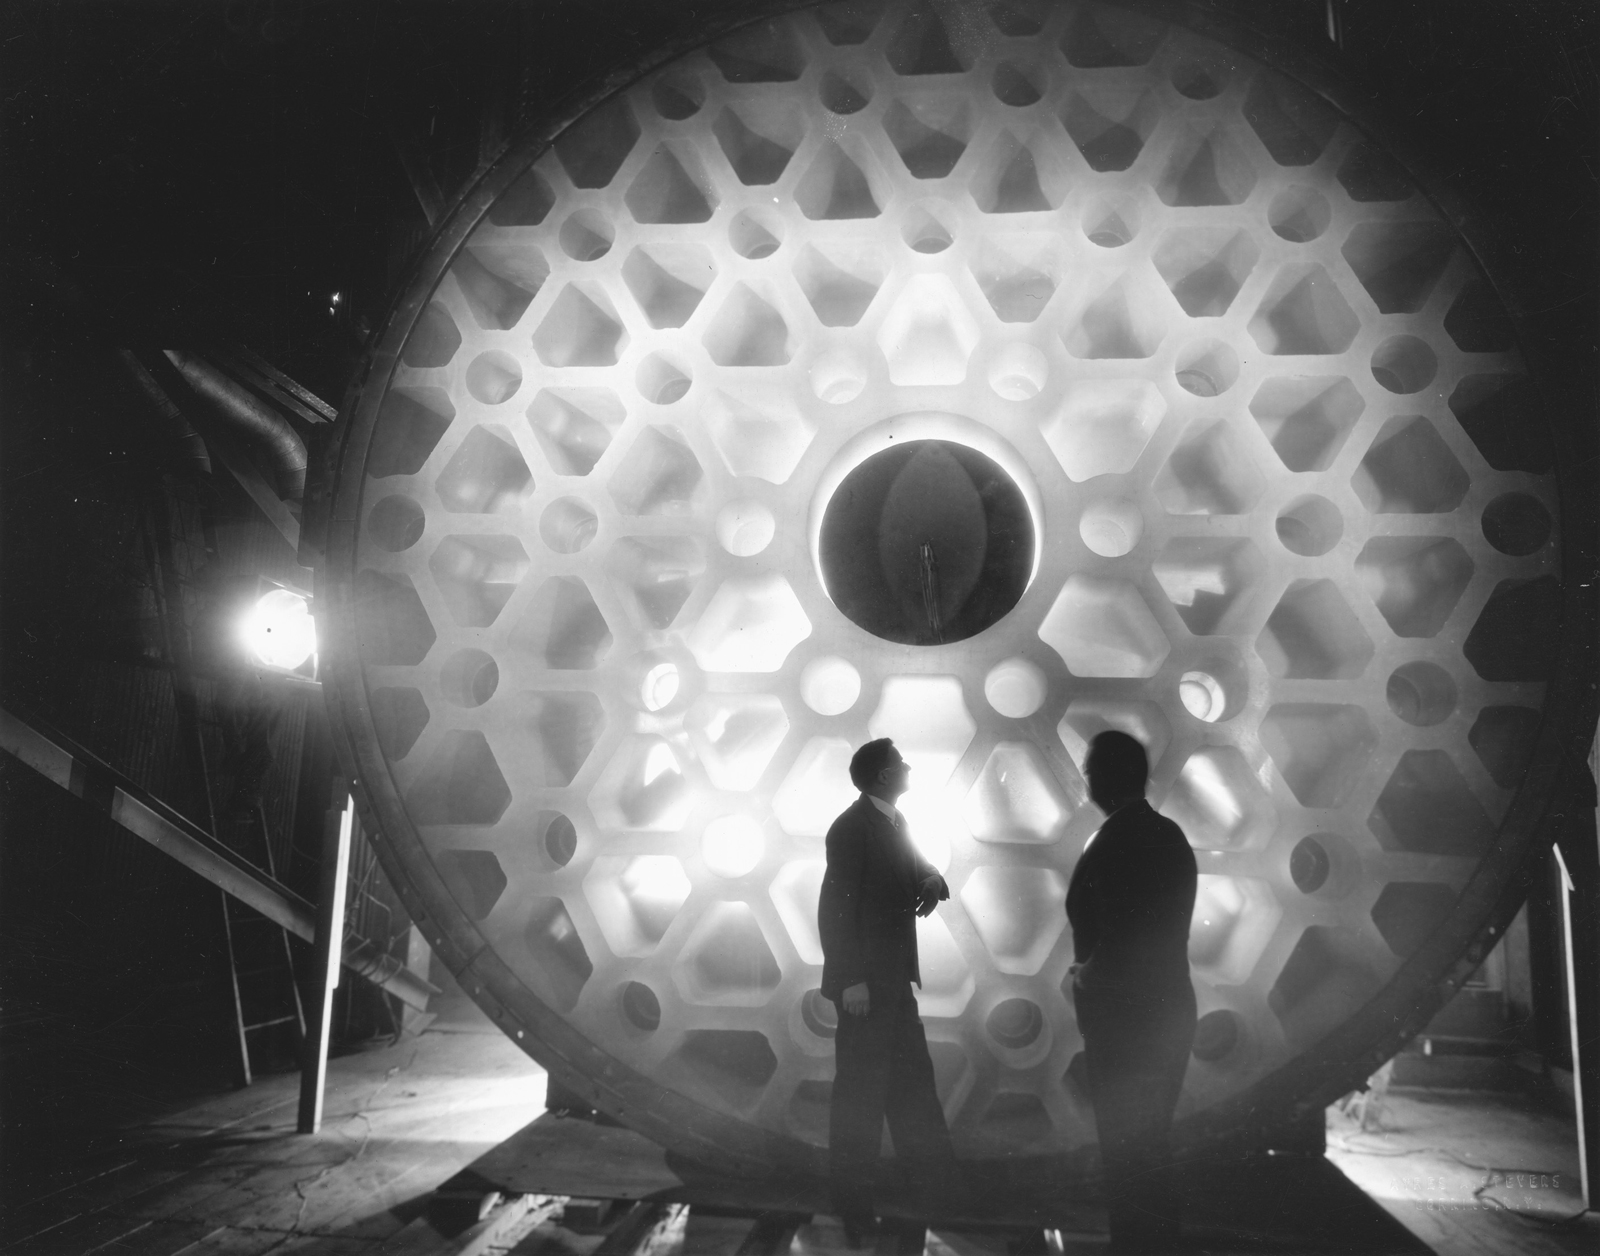
\includegraphics[width=12 cm]{../Figures/twomen}
\caption{Image of the Hale 200-inch (5.1m) primary mirror.  The honeycomb structure was to reduce the mass of the optic and make the surface more ridged}
\label{fig:hale}
\end{figure}


\section{Segmented Mirrors / Active Optics}
In 1977, Dr. Jerry Nelson and a team of scientists at the Lawrence Berkeley National Laboratory, were tasked with designing a 10-meter telescope \cite{BeatingObservatory}.  



\section{FPWFS}



\section{Vector Apodizing Phase Plate}






\begin{itemize}
    \item Segmented Mirrors
    \item FPWFS
    \item vAPP
    % \item hcipy
\end{itemize}



%----------------------------------------------------------------------------------------
%	SECTION 1
%----------------------------------------------------------------------------------------
